\chapter{Analiza problemu}
\thispagestyle{chapterBeginStyle}
\label{rozdzial1}

    W tym rozdziale przedstawiona jest definicja nonogramów oraz sposób ich rozwiązywania.
W kolejnej części rozdziału wypisane są także definicje potrzebne do zrozumienia złożoności problemu,
jakim jest rozwiązywanie nonogramów.



\section{Przedstawienie nonogramów}


\subsection{Opis}
    Nonogramy (znane także jako \textit{Paint by Number} oraz \textit{Picross}) to łamigłówki, w których
celem jest odpowiednie wypełnienie komórek na siatce tak, by uzyskać określony wzór (np. obrazek).
W tym celu należy kolorować pola zgodnie ze wskazówkami umieszczonymi obok każdego wiersza oraz kolumny
na siatce. Wskazówki mają postać ciągu liczb — każda z liczb oznacza ilość wypełnionych komórek z rzędu,
a pomiędzy grupami wypełnionych komórek znajduje się przynajmniej jedna pusta komórka.

    Uściślając powyższą, nieformalną definicję, nonogram to łamigłówka na siatce wielkości $w \times h$,
gdzie $w$ oznacza szerokość planszy wyrażoną w ilości komórek, a $h$ wysokość planszy wyrażoną w
ilości komórek. Dla każdego wiersza i kolumny mamy przedstawiony ciąg liczb $H_n$ będący wskazówką
dla danej linii. Dany element $h_i$ opisuje blok stworzony z $h_i$ wypełnionych komórek z rzędu i, jeśli
$h_i$ nie jest pierwszym elementem ciągu, to blok opisany przez $h_i$ jest oddzielony 
przynajmniej jedną pustą komórką od bloku opisanego przez $h_{i-1}$, 
oraz jeśli $h_i$ nie jest ostatnim elementem ciągu, to blok opisany przez $h_i$ jest oddzielony
przynajmniej jedną pustą komórką od bloku opisanego przez $h_{i+1}$. Linię spełniającą zadaną wskazówkę
opisuje wyrażenie regularne: $l=\text{\^{}}0^*1^{h_1}0^+1^{h_2}0^+\ldots0^+1^{h_n}0^*\text{\$}$, gdzie 
$0$, $1$ oznaczają odpowiednio pustą i wypełnioną komórkę, $h_i$ jest $i$-tym elementem ciągu $H_n$,
będącego wskazówką dla wiersza/kolumny, a $|l| = n$, gdzie $n = w$ dla wiersza i $n = h$ dla kolumny. 
Rozwiązaniem nonogramu jest wypełnienie zadanej planszy w taki sposób, 
by dla każdego wiersza oraz każdej kolumny wskazówki dla nich były spełnione.

\begin{figure}[!htb]
    \centering
    \begin{subfigure}[b]{0.3\textwidth}
        \centering
        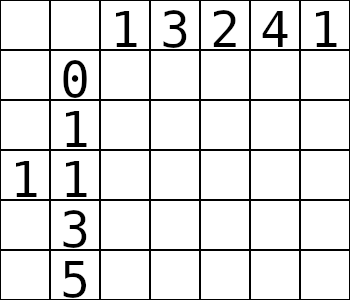
\includegraphics[width=\textwidth]{images/nonogram_example_empty.png}
        \caption{przed rozwiązaniem}
    \end{subfigure}
    \begin{subfigure}[b]{0.3\textwidth}
        \centering
        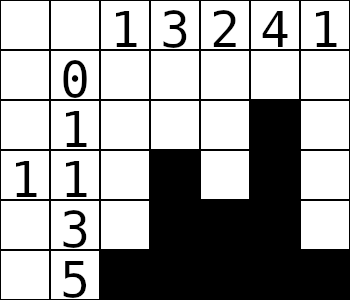
\includegraphics[width=\textwidth]{images/nonogram_example_filled.png}
        \caption{po rozwiązaniu}
    \end{subfigure}
    \caption{Przykładowa plansza}
\end{figure}


\subsection{Definicje}
\begin{definition}
    Wskazówką nazywamy ciąg $H_i$ liczb, opisujący ułożenie wypełnionych komórek w danej linii.
\end{definition}
\begin{remark}
    Dla uproszczenia opisu algorytmów następuje założenie, że pusta linia jest opisywana przez
wskazówkę będącą ciągiem pustym.
\end{remark}
\begin{definition}
    Instancją problemu nonogramu jest czwórka $N = (w, h, R_n, C_n)$, gdzie $w$, $h$ to odpowiednio
szerokość i wysokość planszy, a $R_n$ i $C_n$ są ciągami wskazówek dla wierszy oraz kolumn.
\end{definition}



\section{Wymagane zagadnienia matematyczne}


\subsection{Problem decyzyjny}
\begin{definition}
    Problem decyzyjny to problem, na który odpowiedź stanowi 'tak' lub 'nie'.
\end{definition}
    Problem decyzyjny to pojęcie kluczowe dla klasyfikacji problemu do wybranej klasy złożoności.
By móc sklasyfikować wybrany problem (np. rozwiązanie nonogramu) do jakiejś klasy złożoności,
należy przedstawić go w postaci problemu decyzyjnego.
\begin{example}
    Czy zadany nonogram $N = (w, h, R_n, C_n)$ ma rozwiązanie?
\end{example}


\subsection{Klasa złożoności P}
\begin{definition}
    Klasa złożoności P zawiera wszystkie problemy decyzyjne, których rozwiązanie można znaleźć w czasie wielomianowym.
\end{definition}
\begin{example}
    Znalezienie najkrótszej ścieżki między dwoma punktami w grafie należy do klasy P, ponieważ
algorytm Dijkstry znajduje najkrótszą ścieżkę w czasie wielomianowym. Sformułowanie tego problemu
w postaci problemu decyzyjnego mogłoby brzmieć następująco: Czy dla danego wejściowego grafu $G = (V, E)$
istnieje ścieżka z punktu $v_1 \in V$ do punktu $v_2 \in V$ o długości nie większej niż $x$?
\end{example}


\subsection{Klasa złożoności NP}
\begin{definition}
    Klasa złożoności NP zawiera wszystkie problemy decyzyjne, których rozwiązanie dla odpowiedzi pozytywnej
można zweryfikować w czasie wielomianowym.
\end{definition}
\begin{example}
    Mając zbiór $I$ przedmiotów, gdzie przedmiot $i_n$ to dwójka $(v_n, w_n)$, gdzie $v_n$ to wartość,
a $w_n$ to waga, oraz ograniczenie górne na sumę wag wybranych przedmiotów $w_{max}$, czy można
wybrać przedmioty w taki sposób, by nie przekroczyć limitu wagi $w_{max}$, a by suma wartości
wybranych przedmiotów była większa lub równa $c$?

    Tak zadany problem to wersja decyzyjna problemu plecakowego. Być może nie istnieje algorytm znajdujący
przydział przedmiotów w czasie wielomianowym, ale mając przedstawione rozwiązanie $S \subseteq I$
można zsumować wartości przedmiotów z $S$ i sprawdzić, czy jest to poprawne rozwiązanie.
\end{example}

    Należy zauważyć, że każdy problem z klasy \textit{P} należy także do klasy \textit{NP}, ponieważ
rozwiązanie problemu decyzyjnego jest jednym ze sposobów weryfikacji poprawności jego rozwiązania.
To czy $P = NP$ jest jak do tej pory nierozwiązanym problemem.


\subsection{Redukcja wielomianowa}
\begin{definition}
    Problem A jest redukowalny do problemu B w czasie wielomianowym, jeśli wejścia dla problemu A
można przekształcić na wejścia dla problemu B w czasie wielomianowym, a następnie rozwiązać problem A
wywołując procedurę rozwiązującą problem B wielomianową ilość razy.
\end{definition}
\begin{example}
    Mnożenie liczb $a \cdot b$ można zdefiniować za pomocą operacji dodawania w następujący sposób:
$$a \cdot b = \underbrace{a + a + \ldots + a}_{b}$$
\end{example}
    Należy zauważyć, że jeśli problem \textit{A} jest redukowalny do problemu \textit{B} w czasie wielomianowym,
a problem \textit{B} należy do klasy P, to problem \textit{A} także należy do klasy P, jako że
sposobem na jego rozwiązanie jest użycie redukcji wielomianowej, by traktować go jako instancję problemu \textit{B},
a następnie rozwiązanie go za pomocą algorytmu działającego w czasie wielomianowym.
\begin{corollary}
    Jeśli istnieje redukcja z \textit{A} w \textit{B} w czasie wielomianowym, to \textit{B} jest
co najmniej tak złożony, jak \textit{A}.
\end{corollary}


\subsection{Klasa problemów NP-trudnych}
\begin{definition}
    Problem \textit{H} należy do klasy problemów NP-trudnych, jeśli każdy problem w klasie NP 
jest redukowalny do \textit{H} w czasie wielomianowym.
\end{definition}
    W przypadku klasy problemów NP-trudnych nie ma wymogu, by należące do niej problemy były
problemami decyzyjnymi.
\begin{example}
    Przykładem problemu NP-trudnego jest problem spełnialności (SAT): 'Czy dla danej formuły logicznej
istnieje wartościowanie, dla którego zadana formuła jest spełniona?'. Przynależność tego problemu
do tej klasy została udowodniona w 1971 roku przez Stephena Cooka i Leonida Levina w dowodzie
twierdzenia Cooka-Levina \cite{Cook-Levin}.
\end{example}
    Dla udowadniania przynależności problemu do tej klasy kluczowa jest obserwacja, że istnienie
redukcji wielomianowej z \textit{A} w \textit{B} implikuje przynależność \textit{B} do tej klasy,
o ile \textit{A} także do niej należy.

\subsection{Klasa problemów NP-zupełnych}
\begin{definition}
    Problem decyzyjny \textit{C} należy do klasy problemów NP-zupełnych, jeśli należy do klas problemów
NP-trudnych oraz NP.
\end{definition}
\begin{corollary}
    Pokazanie, że problem decyzyjny \textit{A} jest NP-zupełny sprowadza się do pokazania, że istnieje redukcja
wielomianowa z problemu \textit{H} z klasy problemów NP-trudnych oraz że rozwiązanie problemu \textit{A}
można zweryfikować w czasie wielomianowym.
\end{corollary}



\section{Przypisanie problemu rozwiązania nonogramów do odpowiedniej klasy złożoności}

    Mając zdefiniowane pojęcia potrzebne do klasyfikacji problemu do odpowiedniej klasy złożoności,
należy znaleźć klasę, do jakiej należy rozwiązywanie nonogramów. Z uwagi na specyfikę klas, klasyfikacji
poddana zostanie decyzyjna wersja problemu, tj. 
'\textit{Czy zadany nonogram $N = (w, h, R_n, C_n)$ ma rozwiązanie?}'.


\subsection{Problem rozwiązania nonogramu jest w NP}
    Niech $M_{h, w}$ będzie macierzą oznaczająca rozwiązanie zadanego nonogramu $N = (w, h, R_n, C_n)$,
gdzie $m_{i, j}$ oznacza stan komórki w wierszu $i$ i kolumnie $j$, oraz $m_{i, j} = 1$, jeśli komórka
jest wypełniona, a $m_{i, j} = 0$, jeśli komórka jest pusta. Macierz $M_{h, w}$ jest mapowana na $h + w$ list,
będących ciągami stanów komórek w kolejnych wierszach, i kolumnach.

    Do weryfikacji rozwiązania użyjemy następującej procedury:

\begin{pseudokod}[H]
    %\SetAlTitleFnt{small}
    \SetArgSty{normalfont}
    \KwIn{Lista linii $L$, lista wskazówek $LH$, długość linii $n$}
    \KwOut{Poprawność rozwiązania w osi (\texttt{true/false})}
    \For{$i \leftarrow 1$ \KwTo $|L|$}{
        $Li \leftarrow L[i]$\;
        $Hi \leftarrow LH[i]$\;
        $a \leftarrow 0$\;
        $A \leftarrow []$\;
        \For{$c \in Li$} {
            \If{$c = 1$} {
                $a \leftarrow a + 1$\;
            }
            \Else{
                \If{$a > 0$} {
                    $A.push(a)$\;
                    $a \leftarrow 0$\;
                }
            }
        }
        \If{$a > 0$} {
            $A.push(a)$\;
        }
        \For{$j \leftarrow 1 \KwTo |Hi|$} {
            \If{$A[j] \neq Hi[j]$} {
                \texttt{return false}\;
            }
        }
    }
    \texttt{return true}\;
    \caption{Poprawność rozwiązania w osi}\label{alg:axisValidation}
\end{pseudokod}

    W procedurze \ref{alg:axisValidation} następuje weryfikacja rozwiązania w danej osi. Przykładowo,
wywołując procedurę \ref{alg:axisValidation} dla listy wierszy i ich wskazówek, weryfikujemy Poprawność
rozwiązania w poziomie. Weryfikacja rozwiązania następuje przez wywołanie procedury dwukrotnie,
dla wierszy oraz kolumn. Jeśli w obu przypadkach procedura zwróci \texttt{true}, to rozwiązanie jest poprawne.

    Czas wykonania procedury jest zależny od wielkości planszy. Zewnętrzna pętla wykonuje się
tyle razy, ile jest linii w osi ($h$ w przypadku wierszy, $w$ w przypadku kolumn). Na początku pętli
dochodzi do ekstrakcji pewnych danych do lokalnych zmiennych oraz inicjalizacji tablicy — w zależności
od języka użytego do implementacji, ta grupa operacji zajmuje czas stały bądź liniowy. Następnie
uruchamiana jest pierwsza wewnętrzna pętla. W tej pętli analizowane są dane w danej linii, by zmapować
układ jej komórek do wskazówki, jaką reprezentuje. Złożoność operacji w każdej iteracji jest stała,
jeśli założymy, że powiększenie tablicy o dodatkowy element wymaga stałego czasu — w p.p. czas wykonania
iteracji może być liniowy. Ilość wykonań tej pętli zależy od długości linii.
Po wykonaniu pierwszej pętli, w zależności od układu stanu komórek w linii,
może dojść do kolejnego powiększenia tablicy o dodatkowy element — złożoność nie przekracza liniowej.
Na końcu zewnętrznej pętli wykonywana jest druga pętla, która iteruje po elementach wskazówki zadanej
w rozwiązaniu, i porównuje ich wartość do analogicznych elementów we wskazówce odtworzonej z układu linii.
Rozbieżność oznacza, że rozwiązanie nie jest prawidłowe, i procedura przedwcześnie zakańcza wykonanie.
Długość wskazówki można z góry ograniczyć przez $\lceil \frac{x}{2} \rceil$, gdzie $x$ jest długością
linii.

    Zadana procedura sprawdza poprawność rozwiązania nonogramów, a jej złożoność, w zależności od
implementacji operacji na tablicach, może wynosić $\mathcal{O}(n^2)$ bądź $\mathcal{O}(n^3)$.
Zaproponowana procedura ma złożoność wielomianową, zatem problem decyzyjny rozwiązywania nonogramów
należy do klasy \textit{NP}.


\subsection{Problem rozwiązania nonogramu jest NP-trudny}
    Dowód NP-trudności rozwiązywania nonogramów jest obszerny i wykracza poza zakres tej pracy.
Przykładowy dowód jest opisany w pracy \cite{Nonograms-NP-Hard} i jego zarys jest następujący.
Autor rozpoczyna dowód od powołania się na NP-trudność gry na grafach, nazwanej jako
\textit{Bounded Nondeterministic Constraint Logic}. Następnie, poprzez redukcję, autor udowadnia 
NP-trudność zmodyfikowanej wersji gry, określonej na grafach planarnych. Po udowodnieniu tego faktu
autor konstruuje redukcję wielomianową z planarnej \textit{Bounded Nondeterministic Constraint Logic}
w rozwiązywanie nonogramów, tym samym udowadniając ich przynależność do tej klasy problemów.


\subsection{Problem rozwiązania nonogramu jest NP-zupełny}
    Problem rozwiązania nonogramu został zaklasyfikowany do klasy problemów NP, oraz klasy problemów
NP-trudnych. Wobec tego, rozważany problem należy do klasy problemów NP-zupełnych.
